\documentclass[../main.tex]{subfiles}
\graphicspath{{\subfix{../images/}}}

\begin{document}

Computers need to store data in order to function, like code, or data meaningful to you, like documents and images. Storage devices accomplish this. There are 2 main categories of storage devices, which will be covered here.

\subsection{RAM}
\label{3:sec:ram}

RAM or Random Access Memory; otherwise referred to as just Memory, stores \emph{volatile data} that does not have to be on your hard drive. It only stores data that the computer uses when it is on. Examples of data that goes into memory include temporary values that programs must store; from simple integers to browser tabs. RAM is \textbf{Primary Storage.}

It has a property where it is directly addressable by the CPU. Check section \ref{3:sec:cpu} for details on exactly what that is, but it is essentially the brains of your computer. This makes RAM very fast.

\begin{figure}[H]
    \centering
    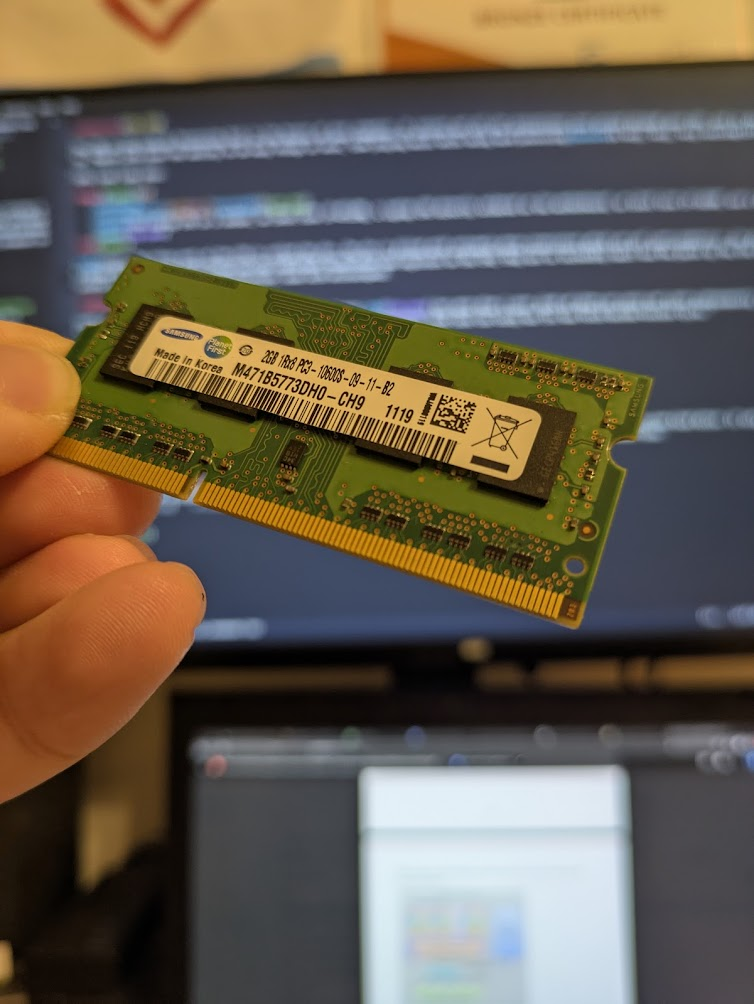
\includegraphics[width=0.5\textwidth]{ram.jpg}
    \caption{What a stick of LPDDR3 RAM (DRAM) looks like.}
    \label{fig:ram}
\end{figure}

Some important information include:

\begin{itemize}
    \item RAM can be freely written to, or read from. The data on RAM can be changed by the user, but not directly; through programs. As an example, opening a browser tab puts data into RAM, but you will not notice physical differences.
    \item RAM is \textbf{\emph{volatile}}. All data stored in it disappears when power to the RAM is lost.
    \item RAM is critical to your computer's function; as all code and data used by code is stored in RAM.
    \item Increasing the amount of RAM will boost the speed of your system, as the computer is able to store more of this temporary data at once in a fast location.
\end{itemize}

There are 2 main kinds of RAM, SRAM (S for static), and DRAM (D for dynamic).

\subsubsection{Dynamic RAM}

DRAM chips (the black squares that you see on the image) consist of transistors and capacitors. It is by far the most common type of RAM in all computers. The access time for DRAM is \textasciitilde60 milliseconds.

They consist of:

\begin{itemize}
    \item Capacitors hold a bit of information (0, or 1)
    \item Transistors act as switches, which allows the chip's control circuitry to read or write to the capacitors.
\end{itemize}

This must be constantly refreshed, as the capacitors cannot hold data for very long.

Benefits of DRAM include:

\begin{itemize}
    \item Much cheaper to make than SRAM
    \item Consume less power on average
    \item They hold a larger total capacity (typically)
    \item DRAM in computers are upgradable in many cases. Modern laptops do not allow you to do so for the most part, but all desktops and some older laptops allow you to remove and exchange DRAM easily for upgrades/repairs.
\end{itemize}

Drawbacks of DRAM include:

\begin{itemize}
    \item It needs constant refreshing to keep the capacitors charged
    \item It is slower than SRAM, by more than 2 times. This limits its applications.
\end{itemize}

\subsubsection{Static RAM}

SRAM chips are made of flip-flops that hold a constant one bit value. They do not need to be constantly refreshed, therefore. SRAM is used when speed is required, such as the CPU's cache. The access time is \textasciitilde25 milliseconds.

Benefits of SRAM include:

\begin{itemize}
    \item Much faster than DRAM due to less latency\footnote{Delay.}
    \item Consumes less power
    \item Does not need to be constantly refreshed
\end{itemize}

Drawbacks of SRAM include:

\begin{itemize}
    \item Much more expensive
    \item Very low capacity
    \item More complex and typically incompatible circuitry must be used to access the RAM.
\end{itemize}

\subsubsection{Differences between DRAM and SRAM}

\begin{longtable}{|p{0.4\textwidth}|p{0.4\textwidth}|}
    \hline 
    \textbf{Dynamic RAM (DRAM)} & \textbf{Static RAM (SRAM)}
    \\ \hline
    DRAM is slower & SRAM is faster
    \\ \hline
    Uses transistors to control the flow of electrons, and capacitors store the binary 1s and 0s & Uses flip-flop circuits
    \\ \hline
    Must be constantly refreshed to make sure the capacitors have charge & Does not need refreshing
    \\ \hline
    Cheaper to make & Much more expensive to make
    \\ \hline
    In a computer, the main memory uses it & The CPU's cache uses it
    \\ \hline
    Less overall power consumption & More overall power consumption
    \\ \hline
    Higher capacity & Lower capacity
    \\ \hline
\end{longtable}

\subsection{ROM}

ROM is like RAM, however, it stands for \emph{read-only memory.} Like RAM (see section \ref{3:sec:ram}), it stores data that is quickly accessible to the computer; i.e. directly addressible by the CPU. However, the \emph{key difference} is that \textbf{ROM is NOT erased when the computer powers off.} This is part of the reason why ROM is purely read-only. ROM cannot be erased.\footnote{Nowadays, computers do not use pure ROM chips anymore, as...they cannot be erased. Instead, they use EEPROM, or electrically-erasable and programmable ROM, which can be erased, but not as easily as RAM. You need a special device to erase an EEPROM, but it is doable. This means that manufacturing errors when making ROM can just be overwritten.}

The main use of ROM in computers is to store the BIOS/UEFI. This is code that the CPU executes immediately when the computer starts up. It does critical checks to make sure all your peripherals are working (like your keyboard), applies specific security patches to your CPU that the CPU maker sees fit, and loads the OS (see section \label{4:sec:the_os_and_kernel}. Increasing the size of ROM does nothing in most systems. ROM is \textbf{Primary Storage.}

\subsection{Virtual Memory}

Virtual Memory is quite a complicated topic. In essence, it is memory made by combining physical RAM and space on your hard drive (HDD or SSD) called the swap space, swap area or swap file to create chunks of memory for each program to use independently.

A diagram illustrates this:

\begin{figure}[H]
    \centering
    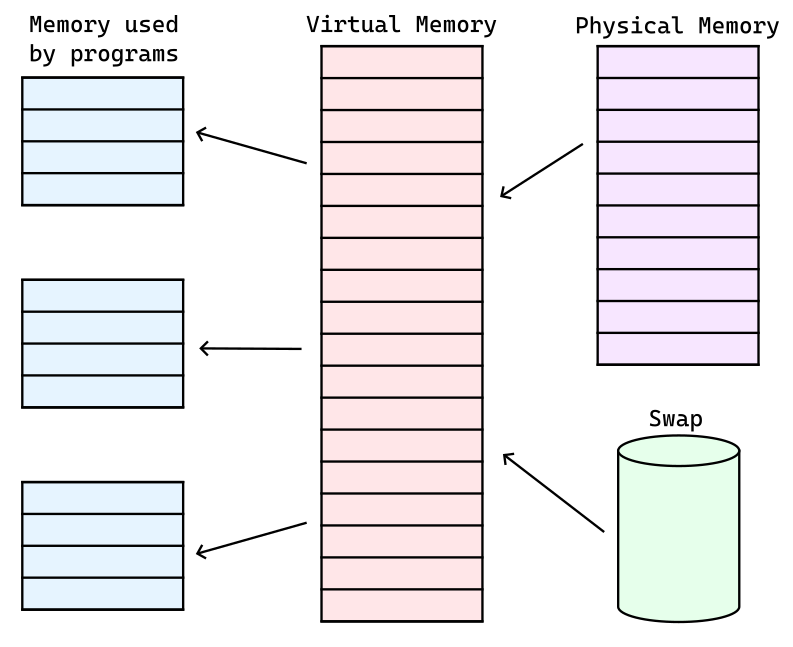
\includegraphics[width=0.7\textwidth]{virtmem.png}
    \caption{A diagram explaining virtual memory.}
    \label{fig:virtmem}
\end{figure}

Each program gets its own slice of the virtual memory, so that memory regions do not accidentially overlap, causing unintended errors. This is also partly for security, so that malicious programs cannot read, say, the passwords in your browser. It is important to note that slices of virtual memory are not all of uniform size. Each slice's location in actual physical memory and in swap may be different.

The process of putting something explicitly into swap memory is called \textbf{paging in}, given one of those chunks in figure \ref{fig:virtmem} is called a page. Moving something out is called \textbf{paging out}.

\subsection{HDDs (Hard disk drives)}

HDDs, Hard Disk Drives or colloquially referred to as spin-drives or just hard drives are \textbf{large secondary storage} devices that has a metal casing and a spinning platter/disc inside of it. The disc inside is magnetized, and the direction at which the tiny magnets points represent binary 0s and 1s

\begin{figure}[H]
    \centering
    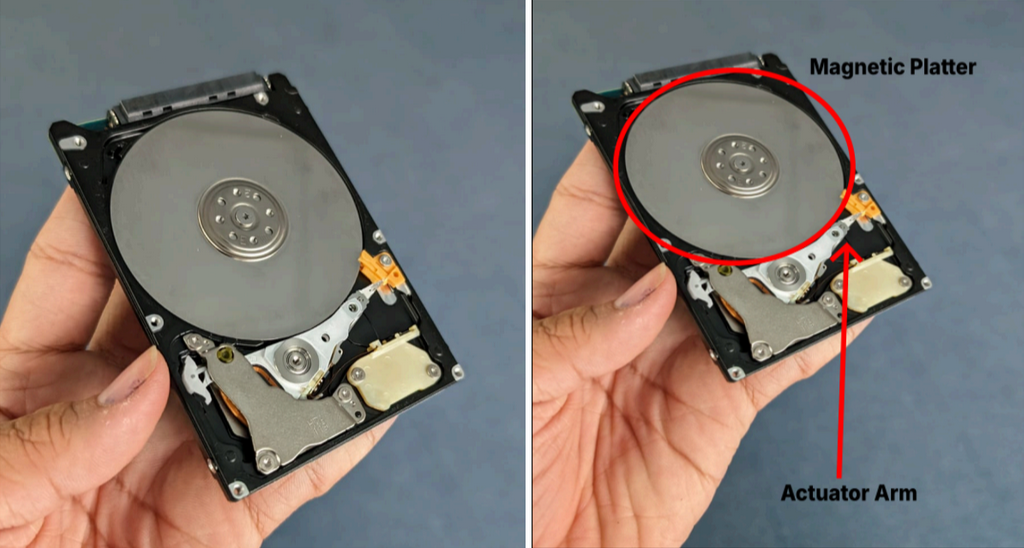
\includegraphics[width=0.7\textwidth]{hdd.png}
    \caption{The inside of an HDD, with annotations explaining the parts.}
    \label{fig:hdd}
\end{figure}

Here are the important components:

\begin{itemize}
    \item The magnetic platter is the medium the data is stored on.
    \item The actuator arm is what actually reads the data off of the medium.
\end{itemize}

These devices typically hold larger amounts of data, such as a lot of films, games, and are used in high-capacity storage devices and security camera backup systems. They can also be used to store the operating system (see section \ref{4:sec:the_os_and_kernel}). Unlike optical media (see \ref{3:sec:optical_media}) hard drive is both the storage device and the medium.

\begin{figure}[H]
    \centering
    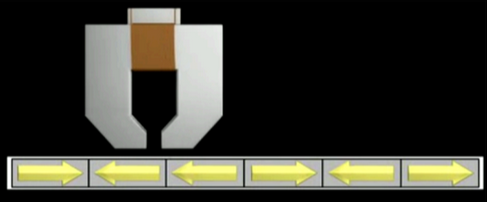
\includegraphics[width=0.5\textwidth]{hdd_magnets.png}
    \caption{What the magnets inside an HDD looks like.}
    \label{fig:hdd_magnets}
\end{figure}

\paragraph{Pros}
\begin{itemize}
    \item They can hold a lot more data than SSDs, as the platters can be manufactured to have more density, along with being able to stack many on top of each other.
    \item They are a lot more affordable (as of 2025, the price gap has decreased by a large margin but still holds true).
\end{itemize}

\paragraph{Cons}
\begin{itemize}
    \item They have a lot of read-write latency (delays when reading or writing data), making one's computer a lot slower\footnote{Only if used as the boot device; the drive at which the OS is stored.}. In short, they are slow.
    \item They are more prone to data rot, which is the corrosion of the platter in the HDD over time.
    \item They have more mechanical parts, making more failure points and making them a lot more fragile.
\end{itemize}

\subsection{SSDs (Solid state drives)}

SSDs or solid state drives, are like HDDs; they can store large amounts of data and are \textbf{secondary storage} devices. Instead of using magnetic discs as the medium, they use NAND flash chips, powered by transistors and NAND gates (see \ref{10:sec:logic_gates}.)

They are typically used in place of HDDs where fast storage is needed; like the startup disk/boot device used to store the operating system, and in mission-critical environments where fast data access is absolutely required. Using these in place of an HDD makes the computer feel snappier as there is no mechanical arm and spinning motor needed to access data.

\begin{figure}[H]
    \centering
    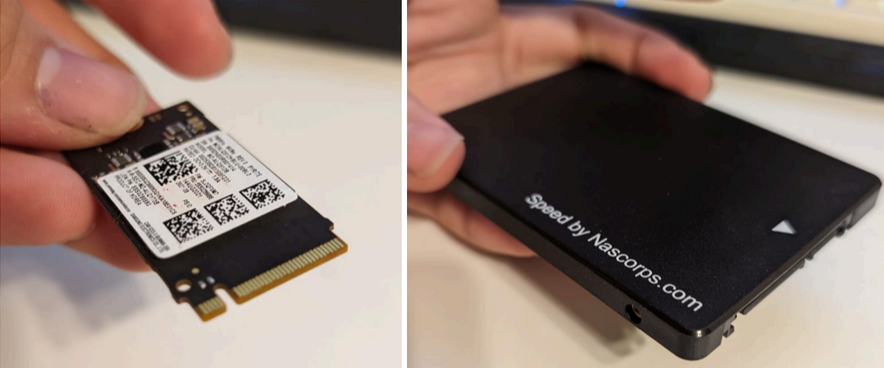
\includegraphics[width=0.7\textwidth]{ssd.png}
    \caption{Two SSDs, one using the NVMe interface and one using SATA. Both are internal drives meant to be mounted into a computer's casing.}
    \label{fig:ssd}
\end{figure}

\paragraph{Pros}
\begin{itemize}
    \item They are much faster than HDDs, as they use non-mechanical NAND flash chips.
    \item They are less prone to data rot; SSDs typically last much longer than HDDs.
    \item They are less fragile than HDDs.
    \item They come in much more form factors and can fit almost everywhere.
\end{itemize}

\paragraph{Cons}
\begin{itemize}
    \item They are more expensive than HDDs.
    \item For backup purposes, they cannot store as much data as HDDs (>10 terabyte capacity SSDs don't really exist as of 2025). Buying smaller drives for backup still does not make sense, as it costs more per terabyte.
    \item Smaller SSDs and faster SSDs generate a lot of heat.
\end{itemize}

\subsection{USB Mass Storage (Flash Drives)}

These are like SSDs, but use a slightly different type of electronic flash chip. They do not consist of many moving parts and can carry small amounts of data in a small form factor. These are intended to be fully external, and uses the universal serial bus (USB, see section \ref{2:sec:usb} for more details). These devices are very commonly seen for software installers that are not fully online, or for moving data through a physical device across computers. Figure \ref{fig:usb_stick} depicts it.

\begin{figure}[H]
    \centering
    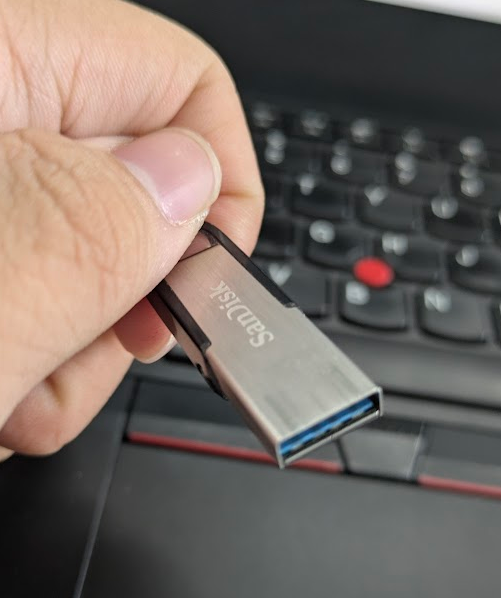
\includegraphics[width=0.4\textwidth]{usb_stick.png}
    \caption{a USB flash drive.}
    \label{fig:usb_stick}
\end{figure}

\subsection{Optical Media (CDs, DVDs, BDs)}
\label{3:sec:optical_media}

Optical media look like discs with a hole in the middle for alignment. Unlike all the other storage devices, optical media just consists of the medium. You need a separate storage device, called an optical drive (or a DVD drive, CD drive etc.) to read them. The shiny side of the disc is what actually holds the data. 

There are 3 types of discs, CDs, DVDs and BDs. CDs hold around 700mb of data, and was made for music. DVDs can hold around 4.7GB of data, and was made for standard definition films (lower resolution). BDs were made recently and is made for very high quality movies. It can hold anywhere between 25 and 100 GB of data. They are shown below:

\begin{figure}[H]
    \centering
    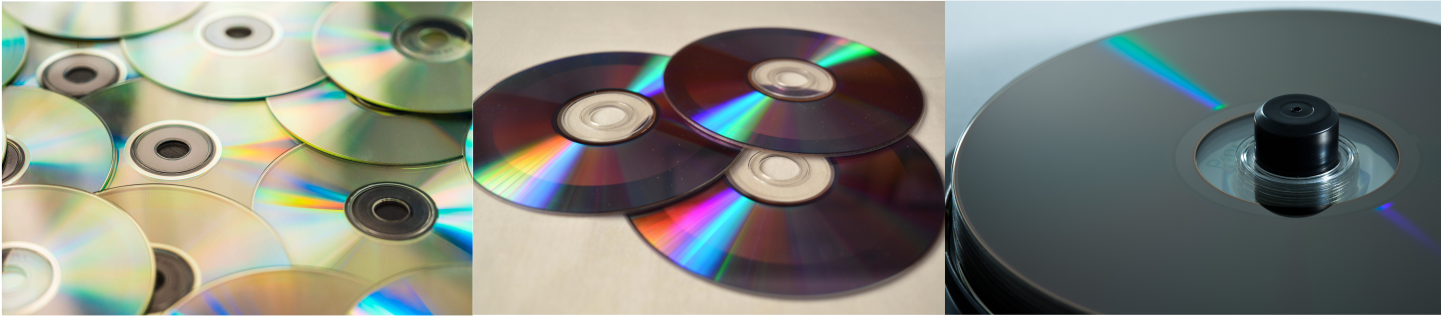
\includegraphics[width=0.9\textwidth]{opticalmedia.png}
    \caption{The back side of CDs, DVDs and BDs respectively.}
    \label{fig:opticalmedia}
\end{figure}

Grooves and flat areas (pits and lands) are used to represent 1s and 0s on optical media. The image that depicts the DVD has a darker area; that is what data written to a DVD looks like. A laser is shone onto the troughs/flat areas, and the reflection angle is measured. Data can only be written to a CD \textbf{ONCE}\footnote{This is called burning.} and cannot be rewritten\footnote{They can, but only for special CDs with the -RW suffix (-RE for blu-rays)}

\subsection{Barcodes}

\begin{figure}[H]
    \centering
    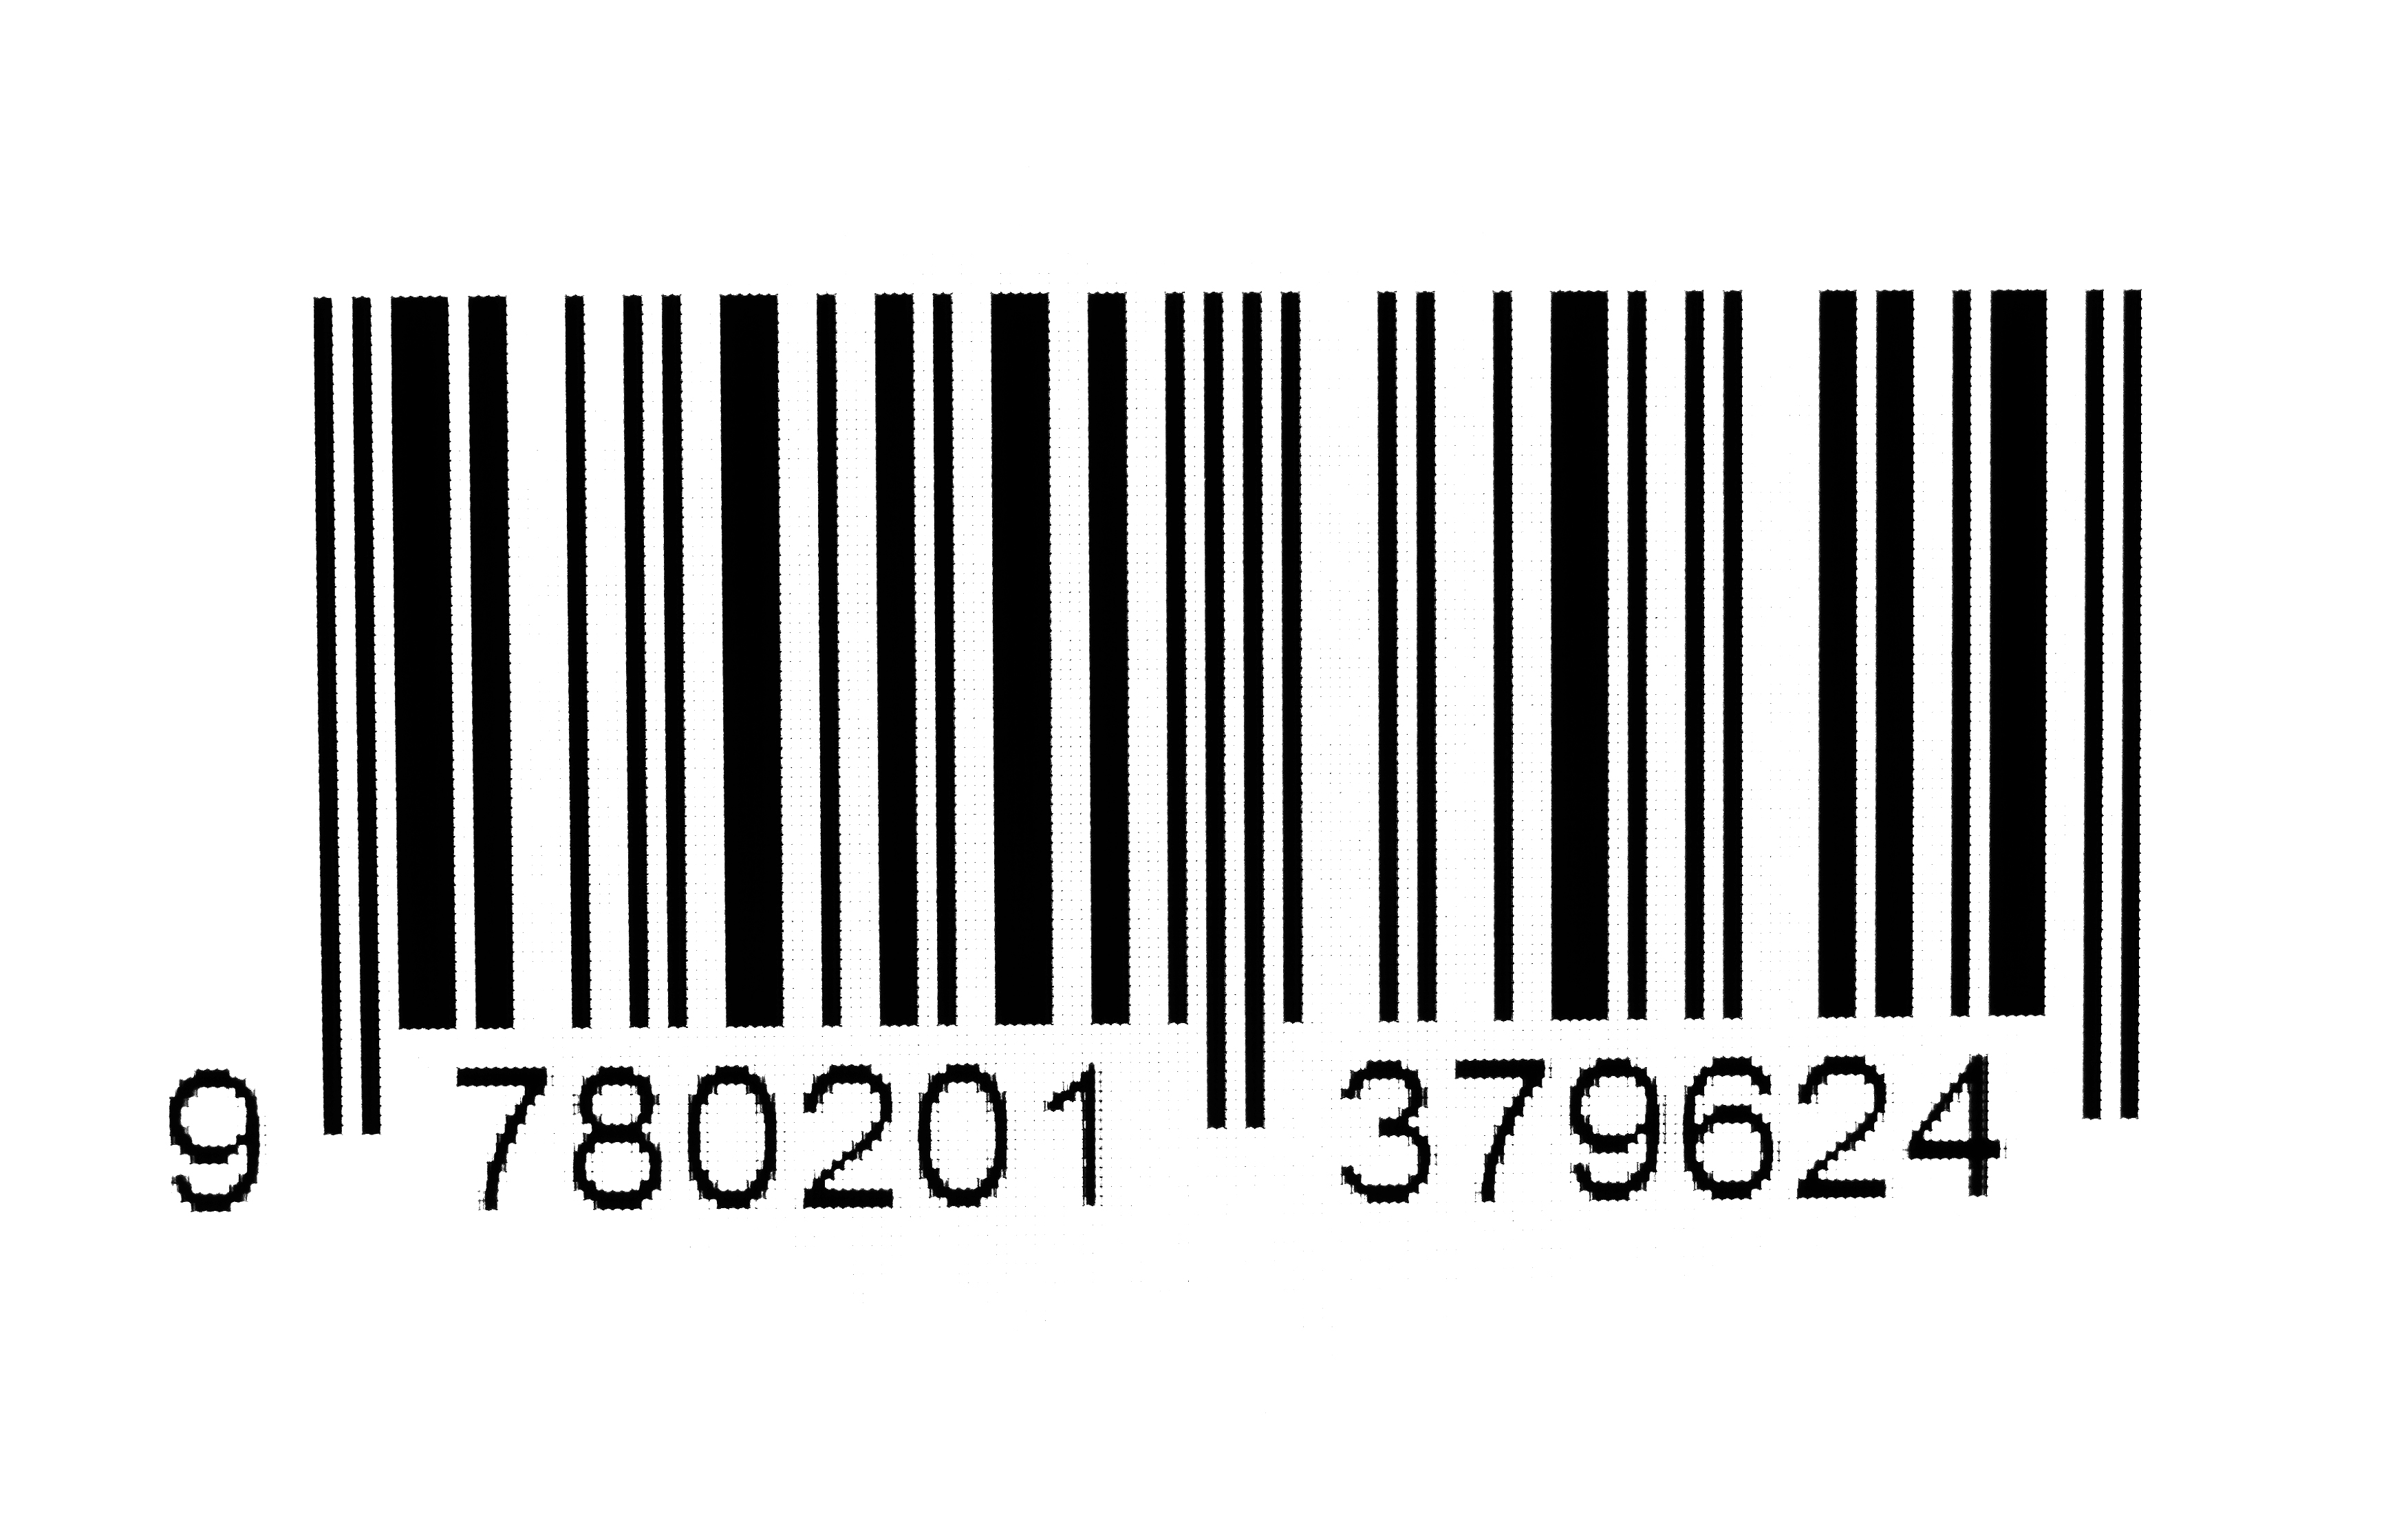
\includegraphics[width=0.6\textwidth]{barcode.png}
    \caption{The back side of CDs, DVDs and BDsrespectively.}
    \label{fig:barcode_again}
\end{figure}

Barcodes are stick shaped codes usually printed on grocery products. They are everywhere; look for a drink bottle or a bag of vegetables; there is likely to be a barcode on it. Each black section represents a 1, and a whte represents a 0. There are 3 sections on the barcode, at the end, the middle and end to align the reader to not read false data.

\subsection{QR Codes}

QR codes are like barcodes, but 2D.

\subsection{Medium vs. Storage Device}
\label{3:sec:medium_vs_storage_device}


\end{document}
